\documentclass[11pt,a4paper]{article}

\usepackage[margin=0.9in,top=0.8in,bottom=0.8in]{geometry}
\usepackage[T1]{fontenc}
\usepackage{helvet}
\renewcommand{\familydefault}{\sfdefault}
\usepackage{courier}
\usepackage{xcolor}
\usepackage{tikz}
\usetikzlibrary{calc,positioning,shapes.geometric,fit,backgrounds}
\usepackage{booktabs}
\usepackage{tabularx}
\usepackage{enumitem}
\usepackage{listings}
\usepackage{fancyhdr}
\usepackage{hyperref}
\usepackage{multicol}
\usepackage{amsmath}
\usepackage{microtype}
\usepackage{colortbl}
\usepackage{ragged2e}
\usepackage{setspace}
\usepackage{parskip}


% ── Color system ──
\definecolor{bg}{HTML}{FFFFFF}
\definecolor{dark}{HTML}{111827}
\definecolor{body}{HTML}{374151}
\definecolor{muted}{HTML}{6B7280}
\definecolor{faint}{HTML}{9CA3AF}
\definecolor{border}{HTML}{E5E7EB}
\definecolor{surface}{HTML}{F9FAFB}
\definecolor{blue}{HTML}{2563EB}
\definecolor{bluelight}{HTML}{EFF6FF}
\definecolor{bluedark}{HTML}{1E40AF}
\definecolor{green}{HTML}{059669}
\definecolor{greenlight}{HTML}{ECFDF5}
\definecolor{purple}{HTML}{7C3AED}
\definecolor{purplelight}{HTML}{F5F3FF}
\definecolor{orange}{HTML}{D97706}
\definecolor{orangelight}{HTML}{FFFBEB}
\definecolor{red}{HTML}{DC2626}
\definecolor{codebg}{HTML}{F3F4F6}
\definecolor{codefg}{HTML}{1F2937}

\pagecolor{bg}
\color{body}

\hypersetup{colorlinks=true,linkcolor=blue,urlcolor=blue}

% ── No page numbers on first pages ──
\pagestyle{fancy}
\fancyhf{}
\renewcommand{\headrulewidth}{0pt}
\fancyfoot[R]{\small\color{faint}\thepage}

% ── Section styles — clean, minimal ──
\usepackage{titlesec}

\titleformat{\section}
  {\fontsize{20}{24}\selectfont\bfseries\color{dark}}
  {\color{blue}\thesection}{0.6em}{}

\titleformat{\subsection}
  {\fontsize{13}{16}\selectfont\bfseries\color{dark}}
  {\color{muted}\thesubsection}{0.5em}{}

\titlespacing*{\section}{0pt}{2.2em}{0.6em}
\titlespacing*{\subsection}{0pt}{1.6em}{0.3em}

% ── Code ──
\lstdefinestyle{code}{
  basicstyle=\footnotesize\ttfamily\color{codefg},
  keywordstyle=\color{blue},
  commentstyle=\color{faint},
  stringstyle=\color{green},
  backgroundcolor=\color{codebg},
  frame=none,
  xleftmargin=12pt,
  xrightmargin=12pt,
  aboveskip=8pt,
  belowskip=8pt,
  breaklines=true,
  columns=fullflexible,
  keepspaces=true,
  morekeywords={fn,let,mut,pub,struct,impl,use,self,Self,trait,for,in,if,else,return,true,false,usize,f32,Vec,Option},
  literate={->}{{$\rightarrow$}}2 {=>}{{$\Rightarrow$}}2,
  aboveskip=0.6em,
  belowskip=0.6em,
}
\lstset{style=code}

% ── Card / box components ──
\newcommand{\card}[1]{%
  \begin{tikzpicture}
    \node[
      rounded corners=6pt,
      fill=surface,
      draw=border,
      line width=0.4pt,
      inner sep=12pt,
      text width=\linewidth-28pt,
    ] {#1};
  \end{tikzpicture}%
}

\newcommand{\accentbar}[1]{%
  \tikz[baseline=(X.base)]{
    \node[inner sep=0pt] (X) {#1};
    \fill[blue] ([xshift=-8pt]X.north west) rectangle ([xshift=-5pt]X.south west);
  }%
}

% ── Stat pill for cover ──
\newcommand{\statpill}[3]{%
  \begin{tikzpicture}
    \node[
      rounded corners=10pt,
      fill=#3,
      inner xsep=14pt,
      inner ysep=10pt,
      minimum width=4.2cm,
      minimum height=1.6cm,
    ] (box) {
      \begin{minipage}{3.6cm}
        \centering
        {\fontsize{24}{28}\selectfont\bfseries\color{dark}#1}\\[2pt]
        {\small\color{muted}#2}
      \end{minipage}
    };
  \end{tikzpicture}%
}

% ── Inline tag ──
\newcommand{\inlinetag}[2]{%
  \tikz[baseline=(T.base)]{
    \node[rounded corners=3pt, fill=#2, inner xsep=5pt, inner ysep=1.5pt] (T)
      {\footnotesize\bfseries\color{#1}\strut};
  }%
}

% ── Clean table style ──
\renewcommand{\arraystretch}{1.35}

\begin{document}

% ══════════════════════════════════════════════════════════════════════
% COVER PAGE
% ══════════════════════════════════════════════════════════════════════
\thispagestyle{empty}

\begin{tikzpicture}[remember picture, overlay]
  % Top accent bar
  \fill[blue] (current page.north west) rectangle ([yshift=-4pt]current page.north east);
  % Subtle grid dots (decorative)
  \foreach \x in {1,2,...,20} {
    \foreach \y in {1,2,...,6} {
      \fill[border] ([xshift=\x*0.95cm, yshift=-\y*0.95cm]current page.north west) circle (0.5pt);
    }
  }
\end{tikzpicture}

\vspace*{3cm}

\begin{flushleft}

{\fontsize{11}{13}\selectfont\color{blue}\texttt{crates/scry-llm} \;\textbullet\; \texttt{v0.1.0}}

\vspace{0.5em}

{\fontsize{42}{48}\selectfont\bfseries\color{dark}scry-llm}

\vspace{0.3em}

{\fontsize{16}{20}\selectfont\color{muted}GPT-2 training from scratch in Rust + CUDA.}

\vspace{0.15em}

{\fontsize{16}{20}\selectfont\color{muted}No PyTorch. No C++. Just \texttt{cudarc} and 10k lines of Rust.}

\end{flushleft}

\vspace{1.8em}

% Stat pills row 1
\noindent
\statpill{10.4k}{lines of Rust}{surface}%
\hfill
\statpill{38}{CUDA kernels}{bluelight}%
\hfill
\statpill{185}{tests passing}{greenlight}%

\vspace{0.7em}

% Stat pills row 2
\noindent
\statpill{50.6\%}{MFU\enspace fp32 + TF32}{purplelight}%
\hfill
\statpill{54.4\%}{MFU\enspace bf16}{orangelight}%
\hfill
\statpill{24h}{from zero to bench}{surface}%

\vfill

\begin{tikzpicture}
  \draw[border, line width=0.4pt] (0,0) -- (\textwidth,0);
\end{tikzpicture}

\vspace{0.6em}

{\small\color{faint}
February 2026\hfill
Rust 1.83+ \;\textbullet\; CUDA 13.0 \;\textbullet\; cudarc 0.19\hfill
MIT / Apache-2.0
}

\newpage

% ══════════════════════════════════════════════════════════════════════
% TOC
% ══════════════════════════════════════════════════════════════════════

\vspace*{0.5em}
{\fontsize{20}{24}\selectfont\bfseries\color{dark}Contents}
\vspace{0.8em}

\makeatletter
\renewcommand{\@dotsep}{200}  % remove dots
\makeatother
{\color{body}\tableofcontents}
\newpage

% ══════════════════════════════════════════════════════════════════════
\section{Overview}
% ══════════════════════════════════════════════════════════════════════

\texttt{scry-llm} is a from-scratch GPT-2 training and inference framework.
The entire forward pass, backward pass, optimizer, and data pipeline are implemented in Rust,
with a custom CUDA backend that compiles 38 NVRTC kernels at runtime and calls cuBLAS for
matrix multiplications.

\vspace{0.8em}
\card{%
\small
\begin{tabularx}{\linewidth}{@{}>{\bfseries\color{dark}}l@{\hspace{1.2em}}X@{}}
Tensor system     & Shape-aware tensors with unique IDs for gradient tracking \\[3pt]
Backend traits    & \texttt{DeviceBackend} + \texttt{MathBackend}\,---\,pluggable CPU / CUDA \\[3pt]
CUDA backend      & 38 custom NVRTC kernels + cuBLAS GEMM with TF32 and bf16 \\[3pt]
Autograd          & Tape-based reverse-mode AD with gradient checkpointing \\[3pt]
Neural modules    & Embedding, Linear, LayerNorm, MHA, MLP, Transformer, GPT-2 \\[3pt]
Optimizer         & AdamW with weight-decay exclusion, cosine LR with warmup \\[3pt]
Training loop     & Gradient accumulation, grad clipping, live MFU reporting \\[3pt]
Inference         & Autoregressive generation with KV cache \\[3pt]
Data pipeline     & Sharded data loader with epoch shuffling \\
\end{tabularx}
}

% ══════════════════════════════════════════════════════════════════════
\section{Architecture}
% ══════════════════════════════════════════════════════════════════════

\subsection{Source Layout}

\vspace{0.3em}
\lstset{
  basicstyle=\footnotesize\ttfamily\color{codefg},
  backgroundcolor=\color{surface},
  xleftmargin=12pt, xrightmargin=12pt,
  aboveskip=6pt, belowskip=6pt,
  frame=none,
}
\begin{lstlisting}
src/
  backend/
    mod.rs         DeviceBackend + MathBackend traits         665 lines
    cpu.rs         CPU reference implementation               687 lines
    cuda.rs        CUDA backend: cuBLAS + NVRTC kernels     2,044 lines
    kernels.rs     38 CUDA kernels (inline C strings)       1,549 lines
  autograd/
    mod.rs         GradTape, SavedData, TapeNode              245 lines
    ops.rs         Differentiable ops: matmul, softmax...     827 lines
    backward.rs    Reverse-mode backward pass                 773 lines
  nn/
    gpt2.rs        Gpt2Config + Gpt2Model                    672 lines
    attention.rs   Multi-head causal self-attention           217 lines
    transformer.rs Transformer block (pre-norm)               180 lines
    embedding.rs   Token + positional embedding               118 lines
    linear.rs      Linear projection                           83 lines
    mlp.rs         2-layer MLP with GELU                       67 lines
    layernorm.rs   Layer normalization
    kv_cache.rs    KV cache for inference                      58 lines
  optim/
    adamw.rs       AdamW optimizer                            119 lines
    scheduler.rs   Cosine annealing with warmup
    clip.rs        Gradient norm clipping                      79 lines
  training.rs      Trainer orchestrator                       427 lines
  data.rs          DataLoader + sharding                      236 lines
  generate.rs      Autoregressive text generation             177 lines
  checkpoint.rs    Safetensors save/load                      195 lines
  tokenizer.rs     BPE tokenizer                              310 lines
\end{lstlisting}

\subsection{Backend Abstraction}

All compute is generic over \texttt{B:\,MathBackend}. Two backends exist:

\vspace{0.5em}
\noindent
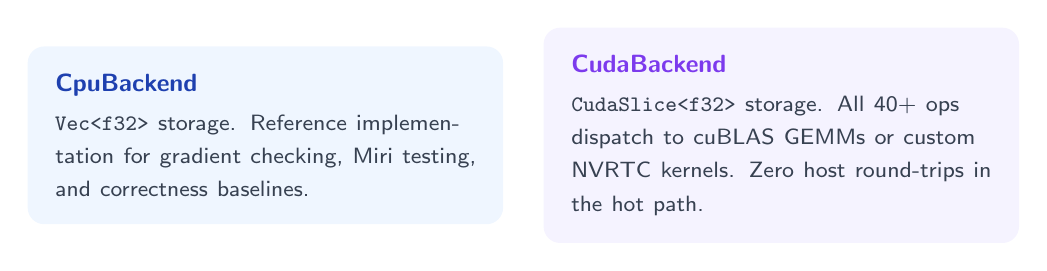
\begin{tikzpicture}
  \node[rounded corners=6pt, fill=bluelight, inner sep=10pt, text width=0.44\textwidth] (cpu) {
    {\small\bfseries\color{bluedark}CpuBackend}\\[2pt]
    {\footnotesize\color{body}\texttt{Vec<f32>} storage. Reference implementation for gradient checking, Miri testing, and correctness baselines.}
  };
  \node[rounded corners=6pt, fill=purplelight, inner sep=10pt, text width=0.44\textwidth, right=0.5cm of cpu] (gpu) {
    {\small\bfseries\color{purple}CudaBackend}\\[2pt]
    {\footnotesize\color{body}\texttt{CudaSlice<f32>} storage. All 40+ ops dispatch to cuBLAS GEMMs or custom NVRTC kernels. Zero host round-trips in the hot path.}
  };
\end{tikzpicture}

\subsection{Autograd}

Reverse-mode automatic differentiation via a \texttt{GradTape}:

\begin{enumerate}[leftmargin=1.8em, itemsep=2pt, label={\color{blue}\bfseries\arabic*.}]
  \item Each \texttt{Tensor<B>} gets a unique \texttt{TensorId} at creation
  \item Forward ops optionally record a \texttt{TapeNode} with saved activations
  \item \texttt{backward()} walks the tape in reverse topological order
  \item Gradient checkpointing trades recompute for memory on marked segments
\end{enumerate}

\subsection{GPT-2 Model}

\vspace{0.3em}
\card{%
\small
\begin{tabularx}{\linewidth}{@{}>{\bfseries\color{dark}}l@{\hspace{1em}}X@{}}
Token embedding     & \texttt{[V,\,D]} lookup --- 50\,257 $\times$ 768 for GPT-2 small \\[3pt]
Position embedding  & \texttt{[T,\,D]} learned --- 1\,024 $\times$ 768 \\[3pt]
Transformer blocks  & Pre-norm: LN $\to$ MHA $\to$ residual $\to$ LN $\to$ MLP $\to$ residual \\[3pt]
LM head             & Weight-tied with token embedding (no duplicate params) \\[3pt]
Residual scaling    & Output projections scaled by $1/\!\sqrt{2L}$ \\
\end{tabularx}
}

% ══════════════════════════════════════════════════════════════════════
\section{CUDA Backend}
% ══════════════════════════════════════════════════════════════════════

\subsection{cuBLAS}

Matrix multiplications dispatch to \texttt{cublasSgemm}\,/\,\texttt{cublasSgemmStridedBatched} for fp32, and \texttt{cublasGemmEx} with \texttt{CUDA\_R\_16BF} inputs for bf16.

\vspace{0.5em}
\noindent
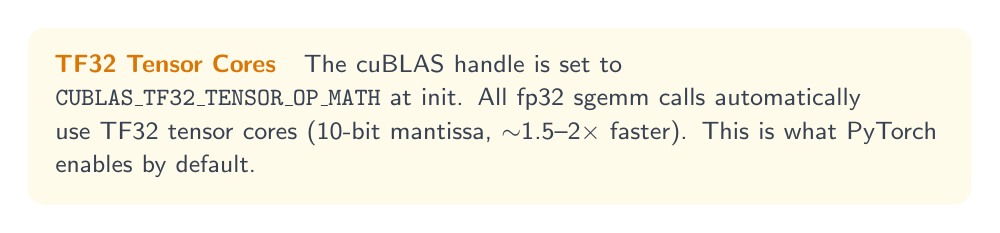
\begin{tikzpicture}
  \node[rounded corners=6pt, fill=orangelight, inner sep=10pt, text width=\linewidth-24pt] {
    {\small\bfseries\color{orange}TF32 Tensor Cores}\quad
    {\small\color{body}The cuBLAS handle is set to \texttt{CUBLAS\_TF32\_TENSOR\_OP\_MATH} at init. All fp32 sgemm calls automatically use TF32 tensor cores (10-bit mantissa, $\sim$1.5--2$\times$ faster). This is what PyTorch enables by default.}
  };
\end{tikzpicture}

\subsection{Custom Kernels\enspace{\normalfont\color{muted}(38 total, NVRTC-compiled at init)}}

\vspace{0.4em}

\begin{tikzpicture}
  \node[rounded corners=6pt, fill=surface, draw=border, line width=0.4pt, inner sep=12pt, text width=\linewidth-28pt] {
    \begin{multicols}{2}
    \small

    {\bfseries\color{blue}Elementwise}\\[2pt]
    {\footnotesize\color{body}
    \texttt{gelu\_fwd/bwd} \;\textbullet\;
    \texttt{scale} \;\textbullet\;
    \texttt{scale\_inplace} \;\textbullet\;
    \texttt{mul\_elementwise} \;\textbullet\;
    \texttt{add\_inplace} \;\textbullet\;
    \texttt{add\_broadcast\_2d} \;\textbullet\;
    \texttt{dropout\_fwd}}

    \vspace{6pt}
    {\bfseries\color{blue}Reductions}\\[2pt]
    {\footnotesize\color{body}
    \texttt{reduce\_sum} \;\textbullet\;
    \texttt{reduce\_rows} \;\textbullet\;
    \texttt{dot\_self} \;\textbullet\;
    \texttt{multi\_dot\_self} \;\textbullet\;
    \texttt{fused\_mul\_reduce\_rows}}

    \vspace{6pt}
    {\bfseries\color{blue}Normalization}\\[2pt]
    {\footnotesize\color{body}
    \texttt{softmax\_fwd/bwd} \;\textbullet\;
    \texttt{layernorm\_fwd/bwd} \;\textbullet\;
    \texttt{cross\_entropy\_fwd/bwd}}

    \vspace{6pt}
    {\bfseries\color{blue}Embedding}\\[2pt]
    {\footnotesize\color{body}
    \texttt{embedding\_fwd/bwd}}

    \columnbreak

    {\bfseries\color{blue}Attention}\\[2pt]
    {\footnotesize\color{body}
    \texttt{causal\_mask\_scale} \;\textbullet\;
    \texttt{batched\_causal\_mask\_scale} \;\textbullet\;
    \texttt{gather/scatter\_columns} \;\textbullet\;
    \texttt{reshape\_bsh\_to\_bnsh} \;\textbullet\;
    \texttt{reshape\_bnsh\_to\_bsh} \;\textbullet\;
    \texttt{flash\_attention\_fwd/bwd}}

    \vspace{6pt}
    {\bfseries\color{blue}Fused Ops}\\[2pt]
    {\footnotesize\color{body}
    \texttt{split\_qkv\_to\_heads} \;\textbullet\;
    \texttt{merge\_heads\_to\_qkv} \;\textbullet\;
    \texttt{fused\_bias\_gelu\_fwd/bwd} \;\textbullet\;
    \texttt{fused\_bias\_dropout\_residual} \;\textbullet\;
    \texttt{residual\_add\_layernorm\_fwd/bwd}}

    \vspace{6pt}
    {\bfseries\color{blue}Optimizer}\\[2pt]
    {\footnotesize\color{body}\texttt{adamw\_step}}

    \vspace{6pt}
    {\bfseries\color{blue}BF16}\\[2pt]
    {\footnotesize\color{body}
    \texttt{f32\_to\_bf16} \;\textbullet\;
    \texttt{bf16\_to\_f32} \;\textbullet\;
    \texttt{flash\_attention\_fwd/bwd\_bf16}}

    \end{multicols}
  };
\end{tikzpicture}

% ══════════════════════════════════════════════════════════════════════
\section{Training Pipeline}
% ══════════════════════════════════════════════════════════════════════

The \texttt{Trainer<B>} struct orchestrates the full loop:

\vspace{0.3em}
\begin{lstlisting}
let config = TrainingConfig {
    batch_size: 32, seq_len: 128, total_steps: 10_000,
    warmup_steps: 200, peak_lr: 3e-4, grad_accum_steps: 4,
    max_grad_norm: 1.0, use_checkpointing: true, ..
};
let mut trainer = Trainer::<CudaBackend>::new(model_config, config);
for step in 0..total_steps {
    let m = trainer.step(&mut loader);  // m.loss, m.mfu, m.tokens_per_sec
}
\end{lstlisting}

\vspace{0.5em}

\noindent
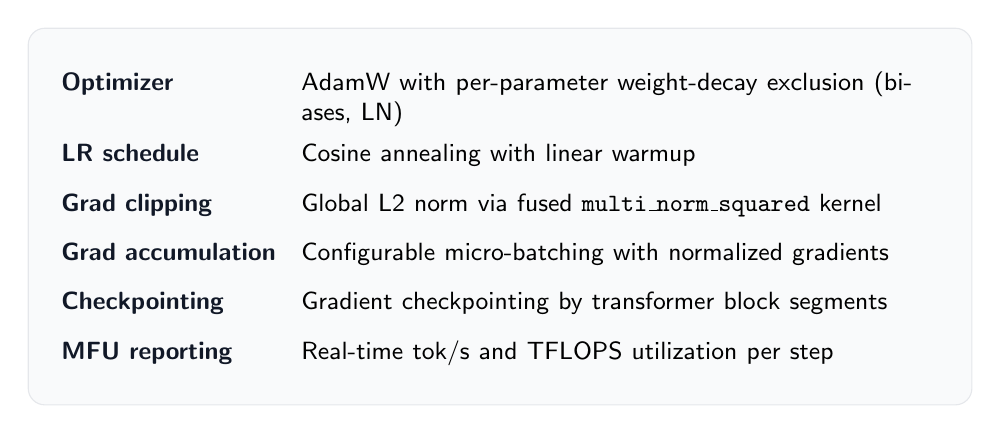
\begin{tikzpicture}
\node[rounded corners=6pt, fill=surface, draw=border, line width=0.4pt, inner sep=12pt, text width=\linewidth-28pt] {
\small
\begin{tabularx}{\linewidth}{@{}>{\bfseries\color{dark}}l@{\hspace{1em}}X@{}}
Optimizer          & AdamW with per-parameter weight-decay exclusion (biases, LN) \\[3pt]
LR schedule        & Cosine annealing with linear warmup \\[3pt]
Grad clipping      & Global L2 norm via fused \texttt{multi\_norm\_squared} kernel \\[3pt]
Grad accumulation  & Configurable micro-batching with normalized gradients \\[3pt]
Checkpointing      & Gradient checkpointing by transformer block segments \\[3pt]
MFU reporting      & Real-time tok/s and TFLOPS utilization per step \\
\end{tabularx}
};
\end{tikzpicture}

% ══════════════════════════════════════════════════════════════════════
\section{BF16 Mixed Precision}
% ══════════════════════════════════════════════════════════════════════

Calling \texttt{init\_gpu\_bf16()} activates mixed-precision mode:

\begin{itemize}[leftmargin=1.5em, itemsep=3pt, label={\color{blue}\textbullet}]
  \item \textbf{Master weights} stay fp32 (full precision for optimizer state)
  \item \textbf{GEMM ops} cast to bf16 on-the-fly via \texttt{cublasGemmEx}
  \item \textbf{FlashAttention} has dedicated bf16 kernel variants
  \item \textbf{Shadow cache} avoids redundant fp32$\to$bf16 casts; invalidated after optimizer steps
  \item \textbf{No loss scaling needed}\,---\,bf16 has 8-bit exponent (same range as fp32)
\end{itemize}

% ══════════════════════════════════════════════════════════════════════
\section{Inference}
% ══════════════════════════════════════════════════════════════════════

Autoregressive generation with KV cache\,---\,only the new token's key/value projections are computed each step.

\vspace{0.3em}
\begin{lstlisting}
let tokens = generate(&model, &prompt_ids, max_new_tokens, temperature, seed);
\end{lstlisting}

% ══════════════════════════════════════════════════════════════════════
\section{Performance}
% ══════════════════════════════════════════════════════════════════════

\vspace{0.1em}
{\small\color{muted}GPT-2 6-layer (81.9M params)\enspace\textbullet\enspace batch\,=\,32, seq\,=\,128\enspace\textbullet\enspace RTX 5070 Ti (23.1 FP32 TFLOPS)}

\vspace{0.8em}

% Performance table as a card
\noindent
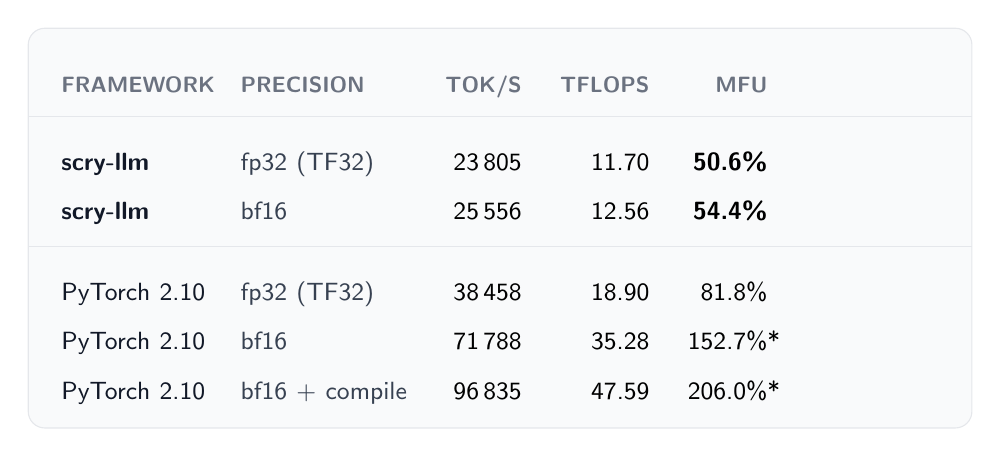
\begin{tikzpicture}
\node[rounded corners=6pt, fill=surface, draw=border, line width=0.4pt, inner sep=0pt, text width=\linewidth-4pt] {
  \small
  \begin{tabularx}{\linewidth}{@{\hspace{12pt}}>{\color{dark}}l@{\hspace{1em}}>{\color{body}}l
    @{\hspace{1.5em}}r@{\hspace{1.5em}}r@{\hspace{1.5em}}r@{\hspace{12pt}}}
  \\[-2pt]
  \rowcolor{surface}
  \bfseries\color{muted}\footnotesize FRAMEWORK &
  \bfseries\color{muted}\footnotesize PRECISION &
  \bfseries\color{muted}\footnotesize TOK/S &
  \bfseries\color{muted}\footnotesize TFLOPS &
  \bfseries\color{muted}\footnotesize MFU \\[4pt]
  \arrayrulecolor{border}\hline\\[-6pt]
  \textbf{scry-llm} & fp32 (TF32)      & 23\,805  & 11.70 & \textbf{50.6\%} \\[3pt]
  \textbf{scry-llm} & bf16             & 25\,556  & 12.56 & \textbf{54.4\%} \\[5pt]
  \arrayrulecolor{border}\hline\\[-6pt]
  PyTorch 2.10       & fp32 (TF32)      & 38\,458  & 18.90 & 81.8\% \\[3pt]
  PyTorch 2.10       & bf16             & 71\,788  & 35.28 & 152.7\%\rlap{*} \\[3pt]
  PyTorch 2.10       & bf16 + compile   & 96\,835  & 47.59 & 206.0\%\rlap{*} \\[6pt]
  \end{tabularx}
};
\end{tikzpicture}

\vspace{0.4em}
{\footnotesize\color{faint}*\,MFU $>$100\% because bf16 tensor-core peak exceeds fp32 ALU peak. Denominator is fp32 TFLOPS for cross-precision comparison (nanoGPT convention).}

\vspace{0.8em}

\noindent
\begin{tikzpicture}
  \node[rounded corners=6pt, fill=bluelight, inner sep=10pt, text width=\linewidth-24pt] {
    {\small\bfseries\color{bluedark}Key takeaways}\\[4pt]
    {\small\color{body}%
    \textbullet\enspace fp32 at 50.6\% MFU = 62\% of PyTorch fp32 throughput. Gap is kernel fusion (\texttt{torch.compile}).\\[2pt]
    \textbullet\enspace Enabling TF32 tensor cores: 32.9\% $\to$ 50.6\% MFU\,---\,a \textbf{1.54$\times$ speedup} from one API call.\\[2pt]
    \textbullet\enspace bf16 at 54.4\% MFU. PyTorch's \texttt{torch.compile} aggressively fuses entire attention blocks.}
  };
\end{tikzpicture}

% ══════════════════════════════════════════════════════════════════════
\section{Test Suite}
% ══════════════════════════════════════════════════════════════════════

{\small\color{muted}185 tests across 20 test files. All passing.}

\vspace{0.6em}

\noindent
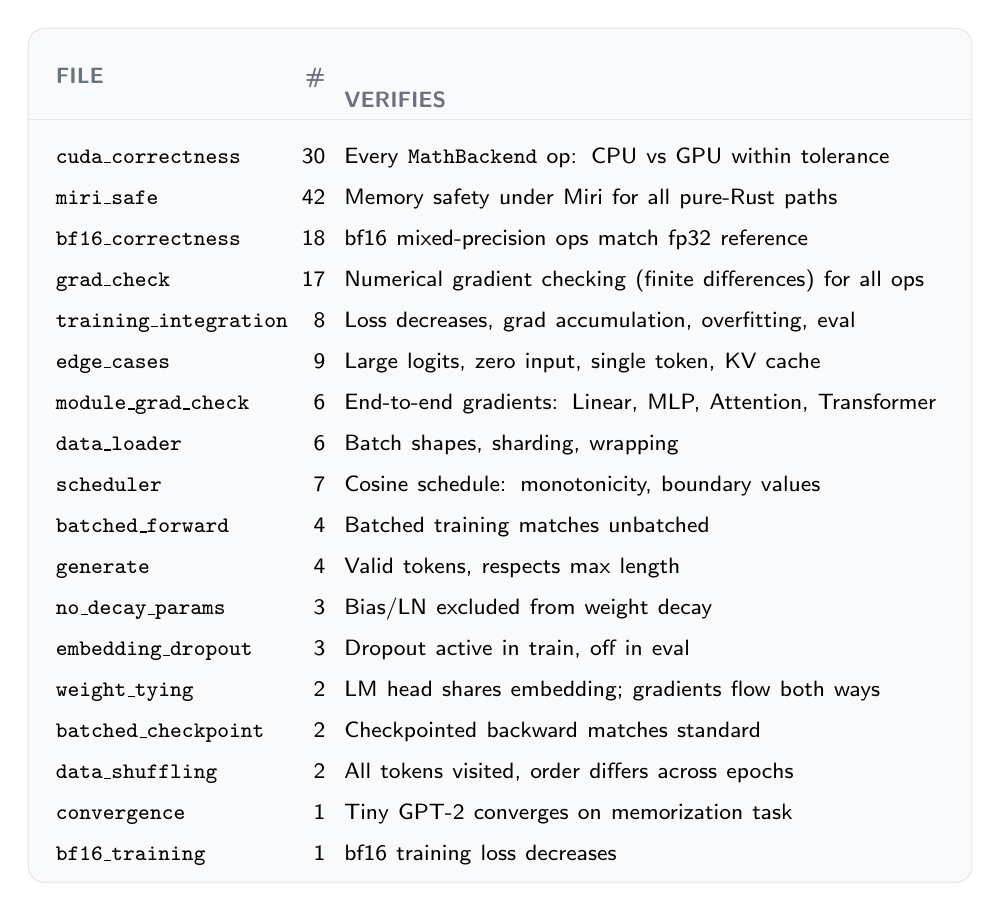
\begin{tikzpicture}
\node[rounded corners=6pt, fill=surface, draw=border, line width=0.4pt, inner sep=0pt, text width=\linewidth-4pt] {
  \footnotesize
  \begin{tabularx}{\linewidth}{@{\hspace{10pt}}l@{\hspace{0.6em}}r@{\hspace{0.8em}}X@{\hspace{10pt}}}
  \\[-2pt]
  \rowcolor{surface}
  \bfseries\color{muted} FILE &
  \bfseries\color{muted} \# &
  \bfseries\color{muted} VERIFIES \\[4pt]
  \arrayrulecolor{border}\hline\\[-6pt]
  \texttt{cuda\_correctness}     & 30 & Every \texttt{MathBackend} op: CPU vs GPU within tolerance \\[2pt]
  \texttt{miri\_safe}            & 42 & Memory safety under Miri for all pure-Rust paths \\[2pt]
  \texttt{bf16\_correctness}     & 18 & bf16 mixed-precision ops match fp32 reference \\[2pt]
  \texttt{grad\_check}           & 17 & Numerical gradient checking (finite differences) for all ops \\[2pt]
  \texttt{training\_integration} &  8 & Loss decreases, grad accumulation, overfitting, eval \\[2pt]
  \texttt{edge\_cases}           &  9 & Large logits, zero input, single token, KV cache \\[2pt]
  \texttt{module\_grad\_check}   &  6 & End-to-end gradients: Linear, MLP, Attention, Transformer \\[2pt]
  \texttt{data\_loader}          &  6 & Batch shapes, sharding, wrapping \\[2pt]
  \texttt{scheduler}             &  7 & Cosine schedule: monotonicity, boundary values \\[2pt]
  \texttt{batched\_forward}      &  4 & Batched training matches unbatched \\[2pt]
  \texttt{generate}              &  4 & Valid tokens, respects max length \\[2pt]
  \texttt{no\_decay\_params}     &  3 & Bias/LN excluded from weight decay \\[2pt]
  \texttt{embedding\_dropout}    &  3 & Dropout active in train, off in eval \\[2pt]
  \texttt{weight\_tying}         &  2 & LM head shares embedding; gradients flow both ways \\[2pt]
  \texttt{batched\_checkpoint}   &  2 & Checkpointed backward matches standard \\[2pt]
  \texttt{data\_shuffling}       &  2 & All tokens visited, order differs across epochs \\[2pt]
  \texttt{convergence}           &  1 & Tiny GPT-2 converges on memorization task \\[2pt]
  \texttt{bf16\_training}        &  1 & bf16 training loss decreases \\[4pt]
  \end{tabularx}
};
\end{tikzpicture}

% ══════════════════════════════════════════════════════════════════════
\section{Dependencies \& Features}
% ══════════════════════════════════════════════════════════════════════

\vspace{0.3em}
\noindent
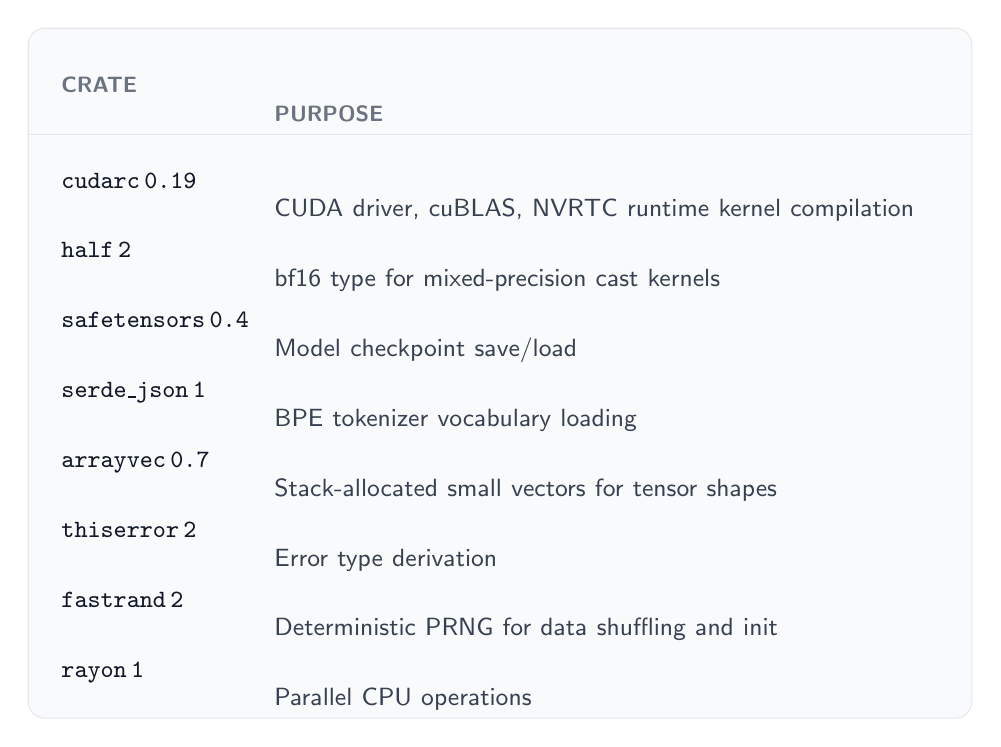
\begin{tikzpicture}
\node[rounded corners=6pt, fill=surface, draw=border, line width=0.4pt, inner sep=0pt, text width=\linewidth-4pt] {
  \small
  \begin{tabularx}{\linewidth}{@{\hspace{12pt}}>{\ttfamily\color{dark}}l@{\hspace{1em}}>{\color{body}}X@{\hspace{12pt}}}
  \\[-2pt]
  \rowcolor{surface}
  \bfseries\color{muted}\sffamily\footnotesize CRATE &
  \bfseries\color{muted}\footnotesize PURPOSE \\[4pt]
  \arrayrulecolor{border}\hline\\[-6pt]
  cudarc\,0.19     & CUDA driver, cuBLAS, NVRTC runtime kernel compilation \\[2pt]
  half\,2           & bf16 type for mixed-precision cast kernels \\[2pt]
  safetensors\,0.4 & Model checkpoint save/load \\[2pt]
  serde\_json\,1   & BPE tokenizer vocabulary loading \\[2pt]
  arrayvec\,0.7    & Stack-allocated small vectors for tensor shapes \\[2pt]
  thiserror\,2     & Error type derivation \\[2pt]
  fastrand\,2      & Deterministic PRNG for data shuffling and init \\[2pt]
  rayon\,1         & Parallel CPU operations \\[4pt]
  \end{tabularx}
};
\end{tikzpicture}

\vspace{0.8em}

\noindent
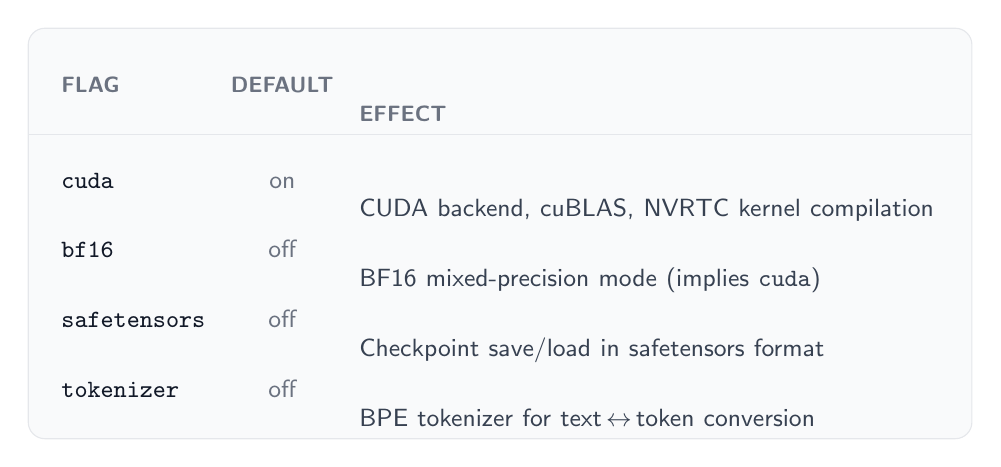
\begin{tikzpicture}
\node[rounded corners=6pt, fill=surface, draw=border, line width=0.4pt, inner sep=0pt, text width=\linewidth-4pt] {
  \small
  \begin{tabularx}{\linewidth}{@{\hspace{12pt}}>{\ttfamily\bfseries\color{dark}}l@{\hspace{1em}}>{\color{muted}}c@{\hspace{1em}}>{\color{body}}X@{\hspace{12pt}}}
  \\[-2pt]
  \rowcolor{surface}
  \color{muted}\sffamily\footnotesize FLAG &
  \bfseries\color{muted}\footnotesize DEFAULT &
  \bfseries\color{muted}\footnotesize EFFECT \\[4pt]
  \arrayrulecolor{border}\hline\\[-6pt]
  cuda         & on  & CUDA backend, cuBLAS, NVRTC kernel compilation \\[2pt]
  bf16         & off & BF16 mixed-precision mode (implies \texttt{cuda}) \\[2pt]
  safetensors  & off & Checkpoint save/load in safetensors format \\[2pt]
  tokenizer    & off & BPE tokenizer for text\,$\leftrightarrow$\,token conversion \\[4pt]
  \end{tabularx}
};
\end{tikzpicture}

\vspace{0.8em}

\noindent
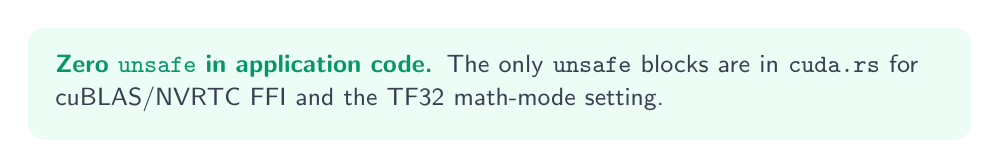
\begin{tikzpicture}
  \node[rounded corners=6pt, fill=greenlight, inner sep=10pt, text width=\linewidth-24pt] {
    {\small\color{green}\bfseries Zero \texttt{unsafe} in application code.}\enspace
    {\small\color{body}The only \texttt{unsafe} blocks are in \texttt{cuda.rs} for cuBLAS/NVRTC FFI and the TF32 math-mode setting.}
  };
\end{tikzpicture}

\vfill

\begin{center}
\begin{tikzpicture}
  \draw[border, line width=0.4pt] (0,0) -- (4,0);
\end{tikzpicture}

\vspace{0.5em}
{\small\color{faint}Built with Rust\enspace\textbullet\enspace\texttt{cudarc} + NVRTC\enspace\textbullet\enspace No C++ dependencies}
\end{center}

\end{document}
